\documentclass[12pt,twoside]{mitthesis}
\usepackage{lgrind}

\usepackage[square,comma,numbers,sort&compress]{natbib}
\usepackage{amsmath,amsthm,amssymb,amsfonts,amsbsy,latexsym}
\usepackage{graphics}
\usepackage{graphicx}
\usepackage{epsfig}
\usepackage[hang,raggedright]{subfigure}
\usepackage{epsf}
\usepackage{setspace}
\usepackage{hangcaption}
\usepackage{graphicx}    % needed for including graphics e.g. EPS, PS
\usepackage{setspace}
\usepackage{multirow}
\usepackage{threeparttable}
\usepackage{cancel}
\usepackage{enumerate}
\usepackage{color}
\usepackage{hyperref}

\hypersetup{
    colorlinks=true,       % false: boxed links; true: colored links
    linkcolor=black,          % color of internal links
    citecolor=black,        % color of links to bibliography
    filecolor=magenta,      % color of file links
    urlcolor=blue           % color of external links
}

\newcommand{\R}{{\mathbb{R}}}
\newcommand{\bit}{\begin{itemize}}
\newcommand{\eit}{\end{itemize}}
\newcommand{\red}[1]{{\color{red}{#1}}}

\graphicspath{{./figures/}}

\begin{document}

%!TEX root = ../main_v01.tex

\title{\large should probably decide whether to include chad's thing...}
%\fontsize{15}{17}\selectfont 
\author{Harriet Li}

\prevdegrees{B.S. Aerospace Engineering (2013)\\
             Massachusetts Institute of Technology}

\department{Department of Aeronautics and Astronautics}
% If the thesis is for two degrees simultaneously, list them both
% separated by \and like this:
% \degree{Doctor of Philosophy \and Master of Science}
\degree{Master of Science}
\degreemonth{June}
\degreeyear{2015}
\thesisdate{May 21, 2015}

%% By default, the thesis will be copyrighted to MIT.  If you need to copyright
%% the thesis to yourself, just specify the `vi' documentclass option.  If for
%% some reason you want to exactly specify the copyright notice text, you can
%% use the \copyrightnoticetext command.  
%\copyrightnoticetext{\copyright IBM, 1990.  Do not open till Xmas.}

% If there is more than one supervisor, use the \supervisor command
% once for each.
\supervisor{Karen Willcox}{Professor of Aeronautics and Astronautics}

% This is the department committee chairman, not the thesis committee
% chairman.  You should replace this with your Department's Committee
% Chairman.
\chairman{Paulo Lozano}{Associate Professor of Aeronautics and Astronautics\\
        Chair, Graduate Student Committee}


% Make the titlepage based on the above information.  If you need
% something special and can't use the standard form, you can specify
% the exact text of the titlepage yourself.  Put it in a titlepage
% environment and leave blank lines where you want vertical space.
% The spaces will be adjusted to fill the entire page.  The dotted
% lines for the signatures are made with the \signature command.
\maketitle

% The abstractpage environment sets up everything on the page except
% the text itself.  The title and other header material are put at the
% top of the page, and the supervisors are listed at the bottom.  A
% new page is begun both before and after.  Of course, an abstract may
% be more than one page itself.  If you need more control over the
% format of the page, you can use the abstract environment, which puts
% the word "Abstract" at the beginning and single spaces its text.

%% You can either \input (*not* \include) your abstract file, or you can put
%% the text of the abstract directly between the \begin{abstractpage} and
%% \end{abstractpage} commands.

% First copy: start a new page, and save the page number.
\cleardoublepage
% Uncomment the next line if you do NOT want a page number on your
% abstract and acknowledgments pages.
% \pagestyle{empty}
\setcounter{savepage}{\thepage}

%Uncomment the following three lines if you want an abstract page
\begin{abstractpage}
Inference problems are often constrained by state equations, which arise from conservation laws, and constitutive relations. Often, a hierarchy of models can be derived from such laws and relations, reflecting varying fidelity versus cost tradeoffs. We introduce a goal oriented, model adaptive, inference algorithm, which allows users to achieve an arbitrary error tolerance, while minimizing the use of high fidelity constraints. Numerical experiments exercise the algorithm on a highly nonlinear inverse problem, and showcase the computational savings and robustness benefits of this new approach.

\end{abstractpage}

% Additional copy: start a new page, and reset the page number.  This way,
% the second copy of the abstract is not counted as separate pages.
% Uncomment the next 6 lines if you need two copies of the abstract
% page.
% \setcounter{page}{\thesavepage}
% \begin{abstractpage}
% Inference problems are often constrained by state equations, which arise from conservation laws, and constitutive relations. Often, a hierarchy of models can be derived from such laws and relations, reflecting varying fidelity versus cost tradeoffs. We introduce a goal oriented, model adaptive, inference algorithm, which allows users to achieve an arbitrary error tolerance, while minimizing the use of high fidelity constraints. Numerical experiments exercise the algorithm on a highly nonlinear inverse problem, and showcase the computational savings and robustness benefits of this new approach.

% \end{abstractpage}

%Uncomment the following three command lines if you want Acknowledgements page
\cleardoublepage

\section*{Acknowledgments}

...

\pagestyle{plain}
\tableofcontents
\clearpage 
\listoffigures
\clearpage
\listoftables
\chapter{Introduction}
...
%------------------------------------------------------------------------------%
\section{Motivation}  %\label{sec:xx}
%------------------------------------------------------------------------------%

In studying the world, physical systems are often represented by mathematical models characterized by a set of parameters; these models are oftentimes partial differential equations (PDEs), and their parameters may be numerous, representing discretized fields. For a given forward model, often based on physical laws and relating the model parameters to predicted observations, one can infer the model parameters based on actual results of these observations \cite{Taran05, BanksKuhn89}. These parameters, especially in engineering contexts, are then used to calculate some Quantity of Interest (QoI).

A given physical system can be represented with varying degrees of fidelity by different models. A high-fidelity model may, for example, take into account more physical laws or be finely discretized, and thus more accurately represent reality; a high-fidelity model is also often more difficult to solve. Since solving the inverse problems generally requires many evaluations of the forward model, it may be cheaper to use a lower-fidelity model, and since the inverse problem is often ill-posed without regularization, it may not be the case that the addition \red{something} of the high-fidelity model is even informed by the observations.

%tarantola seems to frame parameters as independent of forward model; forward model just relates parameters to observables; but in scalar vs field case, parameter choice is part of forward model?

%Inverse problems appear in many contexts. They are difficult to solve because of so and so. In many cases, the purpose of inferring for parameters is to use them to calculate some Quantity of Interest (QoI) that we can then use to make decisions. Goal-oriented approaches trade accuracy in the inferred parameters for accuracy in QoI...?

%------------------------------------------------------------------------------%
\section{Previous Work}  %\label{sec:xx}
%------------------------------------------------------------------------------%
\subsection{Goal-Oriented Approaches}
%goal-oriented DoE from marzouk?
\subsection{Multifidelity Modeling?}

%idea of most-complex \neq best? occam's razor thing from all-hands...
%mixing models? like the thing that inspired vikram to do this model-mixing thing? (stokes-navierstokes...refered to as "classical"...is there a paper?) 
	%what oden,prudhomme,et al refer to as "concurrent" multiscale models; their first numerical example has a lower-fidelity/surrogate model with "homogeneous and deterministic coefficients"
	%other papers with mixed models? "multiscale"? -> "multifidelity"? multimodel - pressure first, then rest as update (typically what this refers to, partankar algorithm); can also think of differently coupled stacks (hierarchies) as different fidelities of models (multiphysics)...
	%poke oden branches for examples?

%------------------------------------------------------------------------------%
\section{Thesis Objectives}  %\label{sec:xx}
%------------------------------------------------------------------------------%
%need to set up the problem we are trying to solve...include LF-HF-MF cartoon? haven't seen other theses with images in intro...
%define inverse problem optimization setup here

%------------------------------------------------------------------------------%
\section{Thesis Outline}  %\label{sec:xx}
%------------------------------------------------------------------------------%



\chapter{Formulation}

In this chapter, we...
%------------------------------------------------------------------------------%
\section{Derivation of Error Estimate}  \label{sec:deriv}
%------------------------------------------------------------------------------%
Given $n_d$ observations $d\in\R^{n_d}$, suppose we wish to infer the parameters $q\in Q$ of a PDE model $a(u,\phi;q)=f(\phi;q),\:\forall\phi\in U$, where $u\in U$ are the states and $U,Q$ are Hilbert spaces. Then this PDE-constrained inverse problem can be written as an optimization problem
\begin{equation}
\begin{array}{r@{}l}
\textrm{Minimize } & \quad J(q)=\frac{1}{2}\|d-C(u)\|_2^2 + R(q) \\ \textrm{s.t. }& \quad a(u,\phi;q)=f(\phi;q),\quad\forall\phi\in U,
\end{array}
\end{equation}
for which the Langrangian is
\begin{equation}
\mathcal{L}(q,u,z)= J(q,u)-(a(u,z;q)-f(z;q)),
\end{equation}
where $z\in U$ is the adjoint. 

Let $\xi=(q,u,z)$ be called the primary variables. Following the work of \cite{BecVex05}, we introduce a set of auxiliary variables $\chi=(p,v,y)\in Q\times U\times U$ corresponding to these primary variables, and define an augmented Lagrangian
\begin{equation}
\mathcal{M}((q,u,z),(p,v,y)) = I(q,u) + \mathcal{L}'(q,u,z)(p,v,y),
\end{equation}
where $I:Q\times U\to\R$ is a functional that gives our QoI. Let $\Psi = (\xi,\chi)$ denote the stationary point of $\mathcal{M}$. Note that
\begin{equation}
\mathcal{M}(\Psi)=I(q,u),
\label{eq:MeqI}
\end{equation} since taking variations of $\mathcal{M}$ with respect to the auxiliary variables recovers the optimality conditions. If we have high-fidelity (HF) and low-fidelity (LF) models for which we can infer parameters, then for each of these we can define an augemented Lagrangian ($\mathcal{M}_{HF}$ and $\mathcal{M}_{LF}$, respectively) with corresponding stationary points $\Psi_{HF}$ and $\Psi_{LF}$. 

Using Equation (\ref{eq:MeqI}), we can write
\begin{equation}
\begin{array}{r@{}l}
I(q_{HF},u_{HF})-I(q_{LF},u_{LF})\: &= \mathcal{M}_{HF}(\Psi_{HF})-\mathcal{M}_{HF}(\Psi_{LF})+\mathcal{M}_{HF}(\Psi_{LF})-\mathcal{M}_{LF}(\Psi_{LF})\textrm{.} 
\end{array}
\end{equation}
Using Equation 21 from \cite{BecVex05}, we can write
\begin{equation}
\mathcal{M}_{HF}(\Psi_{HF})-\mathcal{M}_{HF}(\Psi_{LF}) = \frac{1}{2}\mathcal{M}'_{HF}(\Psi_{LF})(\Psi_{HF}-\Psi_{LF})+\mathcal{R}(e^3)\textrm{,}
\label{eq:preadj}
\end{equation}
where $e=\Psi_{HF}-\Psi_{LF}$. We cannot solve for $\Psi_{HF}$, and we cannot replace $\Psi_{HF}-\Psi_{LF}$ with an interpolation estimate as was done for $\Psi-\Psi_h$ in \cite{BecVex05}, since we now have different models instead of different discretizations of the same model. 

We take an adjoint approach to obtain the term $\frac{1}{2}\mathcal{M}'_{HF}(\Psi_{LF})(\Psi_{HF}-\Psi_{LF})$ by viewing it as an error in a linear output. As $\Psi_{HF}$ is a stationary point, it satisfies $\mathcal{M}'_{HF}(\Psi_{HF})(\Phi)=0$. Let its variational form be
\begin{equation}
A_{HF}(\Psi_{HF},\Phi)=F(\Phi),\:\forall\:\Phi\in(Q\times U\times U)^2,
\end{equation}
and define an output 
\begin{equation}
\mathcal{Q}(\Psi_{HF})=\mathcal{M}'_{HF}(\Psi_{LF})(\Psi_{HF}).
\end{equation}
We can then solve
\begin{equation}
A_{HF}(\Phi,\Lambda)=\mathcal M'_{HF}(\Psi_{LF})(\Phi),\:\forall\:\Phi\in(Q\times U\times U)^2
\label{eq:superAdjEq}
\end{equation}
for the adjoint $\Lambda$, which can be used to obtain
\begin{equation}
\mathcal M'_{HF}(\Psi_{LF})(\Psi_{HF}-\Psi_{LF})=\mathcal{M}'_{HF}(\Psi_{LF})(\Lambda).
\label{eq:adjOutErr}
\end{equation}
Combining Equations (\ref{eq:preadj}) and (\ref{eq:adjOutErr}) and dropping the higher-order term $\mathcal{R}(e^3)$, we obtain an expression for the error in the QoI from inferring the parameters of a low-fidelity model instead of a high-fidelity model:
\begin{equation}
I(q_{HF},u_{HF})-I(q_{LF},u_{LF})\approx\frac{1}{2}\mathcal{M}'_{HF}(\Psi_{LF})(\Lambda)+\mathcal M_{HF}(\Psi_{LF})-\mathcal M_{LF}(\Psi_{LF}).
\label{eq:finErrExp}
\end{equation}
%there is a minus sign in the adjoint-weighted residual expression in vikram's writeup...but not in any of your stuff...looks like that depends on how you define the residual...Ax-b or b-Ax...should you define that somewhere?

The equations in this section apply also when the low-fidelity model is replaced with an intermediate model. Just as \red{error estimates} can be used to guide mesh-refinement, Equation (\ref{eq:finErrExp}) can be decomposed into elemental contributions and used to guide the creation of a mixed-fidelity model, where the high-fidelity model is used in some parts of the domain, and the low-fidelity model is used in the rest. The error estimate (\ref{eq:finErrExp}) can be calculated again, using the mixed-fidelity model as the lower-fidelity model; this process can be repeated, successively increasing the proportion of the domain in which the high-fidelity model is used, until some threshold is reached. %should you expand this into an "algorithm"-type section? section/note that forming a mixed-fidelity model is not always so straightfoward? should poke literature about how this is done if so (model interfacing that Oden,Prudhomme, etal talk about...also seemed to have a sort of interior-boundary-condition for stokes-ns mix)...also include de-refinement? (choices of how to pick where to refine? if so, would we need to reference other papers where similar choices are made?)

%do we have restrictions on I? the prediction process could be a whole 'nother PDE, or something as simple as our subdomain integral...needs to be at least once differentiable? with respect to? B+V just seems to have I' with respect to state, even though I(q,u)...B+V only say that I is some functional...if I is a PDE, then is it also possible that it can be excessively complex as well?

%------------------------------------------------------------------------------%
\section{Limitations and Bounds}  %\label{sec:xx}
%------------------------------------------------------------------------------%

The error estimate (\ref{eq:finErrExp}) is exact in the case where the model PDEs and QoI functional are linear. In the presence of nonlinearities, the error estimate is approximate, due to having dropped the higher order terms $\mathcal{R}(e^3)$, and due to the need to linearize about $\Psi_{HF}$ in forming the adjoint problem (\ref{eq:superAdjEq}). It will also sometimes be the case that it is cheaper to solve the inverse problem with the high-fidelity model than to calculate the quantities needed to build up to a mixed-fidelity model for which the estimated error in the QoI is acceptably low. %bounds on accuracy of error estimate? B+V doesn't say anything about bounds on the third order term...I think FE stuff can say things about e in mesh-discretization case but not for different models...if we can't come up with bounds, can we just acknowledge that as a current weakness? did oden+prudhomme have bounds? (no) 	-> there haven't really been anything published on e for multiple-models...hence why we want as high an order method as possible...perhaps once there is a defined hierarchy (poke model hierachy?), as there is for mesh-refinement, perhaps then...otherwise models could be totally unrelated...

The two models must also have a weak form, so this cannot be applied to, for example, a model of chemical reactions using kinetic Monte Carlo. The lower-fidelity model could, for example, be a simplified model including fewer physical phenomena, be a reduced-order model, or have a reduced parameter space. The two models could also correspond to two levels of mesh-refinement, though in this case the method described in \cite{BecVex05} would be more efficient, since interpolation could be used to estimate $\Psi_{HF}-\Psi_{LF}$ instead. The two models must also have some degree of compatibility, in that the variables of one model must have some meaning in the other. %is this something to expand on, or just give the weak form assumption and leave it at that?

%in the formulation, psiLF and psiHF share the same space...which they might not necessarily be able to be made to if psiMF has discontinuities allowed but psiHF doesn't?

%cost analysis?
	%assume LF inverse problem is cheap to solve; if we solve for auxiliary naively (not B+V's) way, then so and so many linear solves...? anything we can do for superadj other than breaking into blocks?

%more than two models? the error breakdown is only ever for two models at a time...if A>B>C, then first do between B and C, get a mix of B+C as your new 'LF', then do between B+C and A?

%%%%

%How different can the models be before the error estimate becomes unreliable? Are there any kinds of PDEs for which the error estimate is unreliable? (in forward problems, adjoint based error estimation works well for any adjoint consistent formulation; handles hyperbolic and highly nonlinear problems well (Darmofal has a paper comparing it to other methods for hyperbolic problems?); possible that this might extend to our case, though having an inverse problem might screw that up; might have to settle for running numerical experiments on simplified versions to build/decrease confidence that it would work on more complex version)

%How much of an issue would adjoint inconsistency be? (Perhaps not so much in gradient calculation in solving inverse problem, since you want to find an optimum for a particular choice of model and mesh, but it gets worse when you want to do things like mesh refinement, since then adjoint-of-discrete not corresponding to discretized-adjoint breaks up your connection to the infinite dimensional system; in our case, we are comparing two models with set discretizations, and there is no continuous ideal that we need to relate to...)

%transient case? theory should hold, since we can stack solutions at time-steps into one giant solution and theoretically solve everything in one go; should we discuss how that would be implemented though? states evolve forward, adjoints evolve backwards, auxiliary are linearly related to primary...do people automatically think of steady-state when they see a(*,*)=f(*) form? B+V's example is steady-state...but weak form can definitely encapsulate transient (DG_NonLinearSystems, slide 8) -> writing out steps for transient case doesn't really add anything to this theory; enough existing literature to see how to implement in transient case

%in B+V, they say "The form a and the observation C are assumed to be three times continuously differentiable"...what might a not-differentiable operator look like? should we include this in assumptions about form? (their C is observation operator acting on state, not params) why three times? (for HOT remainder)

\chapter{Numerical Results}

For simplicity of implementation, we demonstrate the results using pairs of steady-state models sharing the same states, mesh, and basis functions.

%------------------------------------------------------------------------------%
\section{Convection-Diffusion and Convection-Diffusion-Reaction Models}  %\label{sec:xx}
%------------------------------------------------------------------------------%

In this section, we demonstrate the method derived in Section \ref{sec:deriv} for two models in a 2D domain. In this case, the two models differ in the physics modeled. The high-fidelity model 
\begin{equation}
k_d\nabla^2 u - \vec{V}\cdot\nabla u + k_ru^2= f(q)
\end{equation}
is described by a single-species convection-diffusion-reaction equation with a nonlinear reaction term, where $k_d = 0.1$ is a diffusion coefficient and $k_r = -42.0$ is a reaction coefficient. The low-fidelity model
\begin{equation}
k_d\nabla^2 u - \vec{V}\cdot\nabla u + k_ru^2= f(q)
\end{equation}
differs only in the removal of reaction term. The velocity is described by $\vec{V}(x,y) = (2y(1-y),0)$, with the Peclet number everywhere in the domain $\Omega=[0,5]\times[0,1]$ small enough to make stabilization unnecessary. Homogeneous Dirichlet boundary conditions are used for simplicity. 

Given observations $d=(u(0.35,0.35),u(1.56,0.61),u(3.1,0.5))$ from three points in the domain, we wish to infer the forcing field $f(q)=q$ in order to calculate
\begin{equation}
I(q,u)=\int_{(x,y)\in \Omega_I} u \:\textrm{d}A,
\end{equation}
where $\Omega_I=[0.625,0.875]\times[0.375,0.625]$. The locations of the observations and the region $\Omega_I$ over which the QoI is calculated is shown in Figure \ref{fig:baseSetup}. Since the inverse problem is ill-posed, a Tikhonov regularization term $\frac{\beta}{2}\int_\Omega \|\nabla f(q)\|_2^2\:\textrm{d}A$ is used.

\begin{figure}[h]
\centering
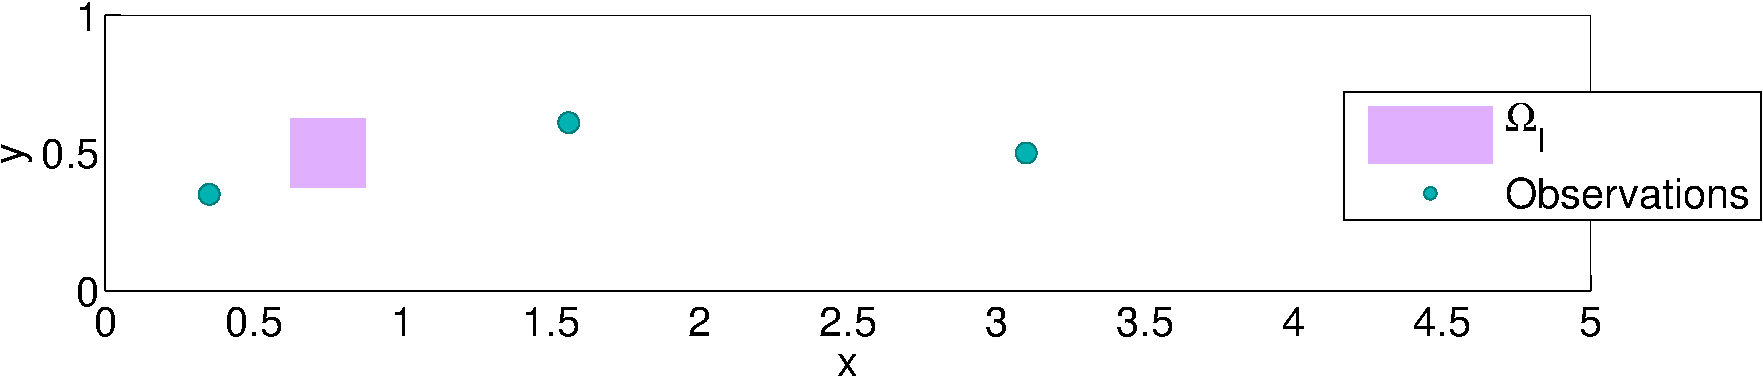
\includegraphics[width=0.8\textwidth]{baseSeries/setup_3_3.pdf}
\caption{Locations of observations and QoI region \red{ADD X TO AXIS...}}
\label{fig:baseSetup}
\end{figure}

Using the element-wise decomposition of (\ref{eq:finErrExp}), the proportion of the domain in which the high-fidelity model is used is increased until the estimated absolute relative error in the QoI is less than $1\%$. Figure \ref{fig:baseRef} shows the element-wise decomposition of the error estimate, as well as the areas of the domain where the low- and high-fidelity models were used. The true and estimated absolute relative errors in the QoI for these same intermediate models are shown in Figure \ref{fig:baseErr}, while the relative error in the error estimate is shown in Figure \ref{fig:baseErrErr}. %or effectivity index, since that's a standard for error estimates?
It can be seen that in this case, while the error estimates are not exact due to the nonlinear reaction term in the high-fidelity model, the error estimates are fairly accurate, and the QoI that would have been obtained from solving the inverse problem with the high-fidelity model can be replicated to within $1\%$ with a mixed-fidelity model where the high-fidelity model is used in only $20\%$ of the domain.

\begin{figure}[h]
\makebox[\textwidth]{%
    \begin{minipage}[t]{0.65\textwidth}
      \centering
      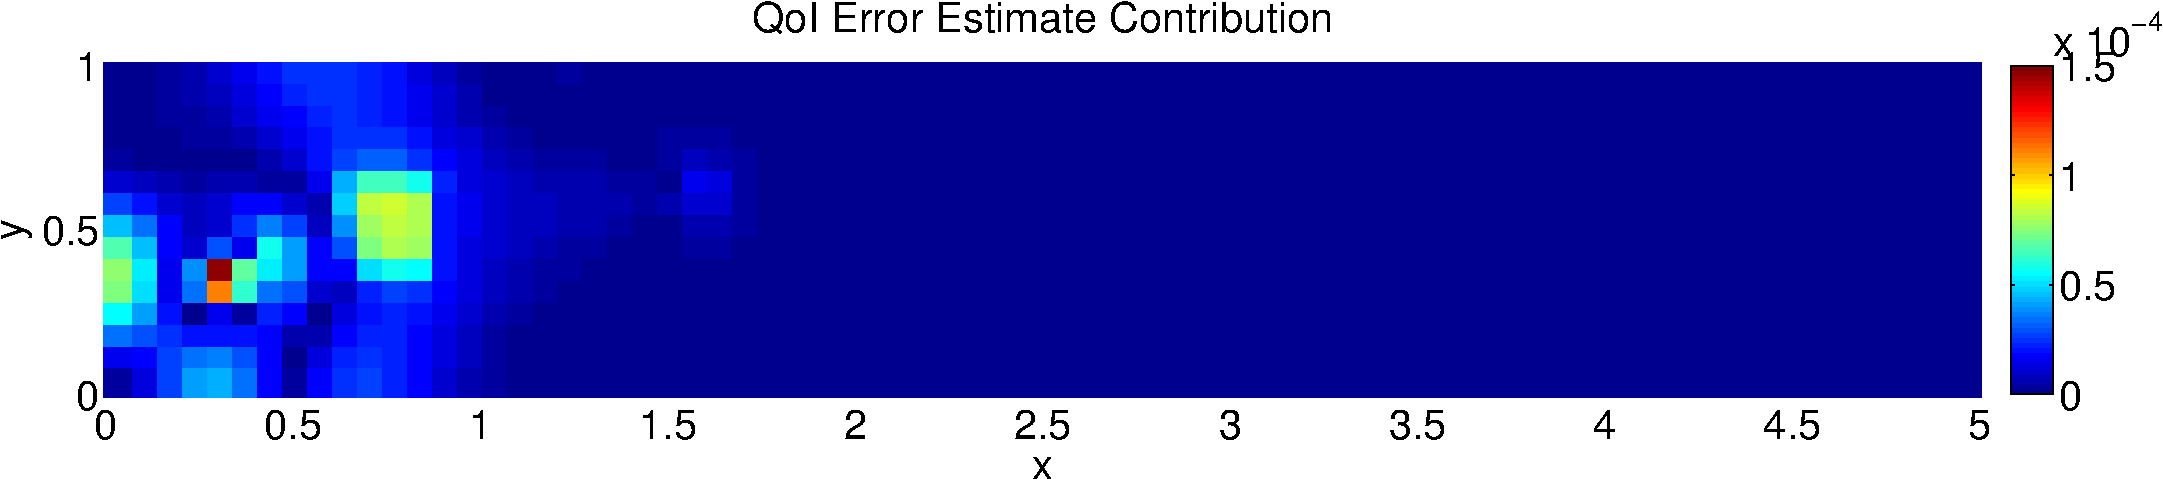
\includegraphics[width=\textwidth]{baseSeries/err_breakdown_LF.pdf}
    \end{minipage}%
    \hfill
    \begin{minipage}[t]{0.62\textwidth}
      \centering
      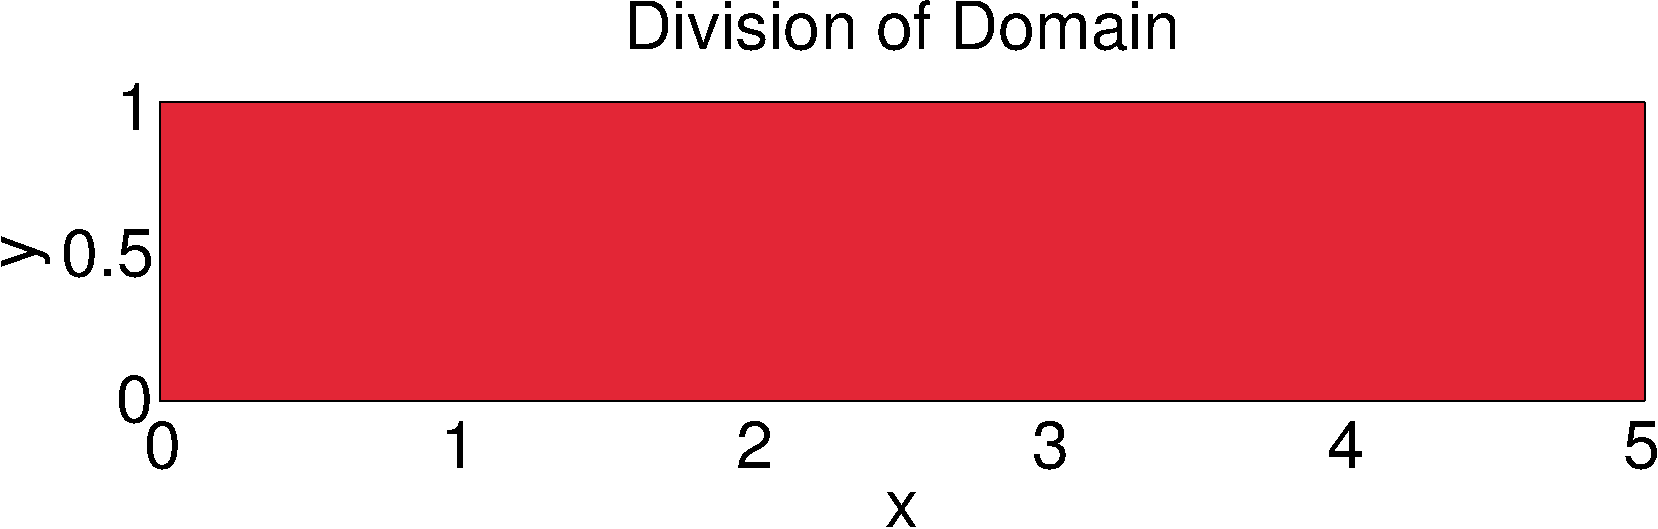
\includegraphics[width=\textwidth]{baseSeries/cd_cdr_LF_divvy.pdf}
    \end{minipage}%
    }
\makebox[\textwidth]{%
    \begin{minipage}[t]{0.65\textwidth}
      \centering
      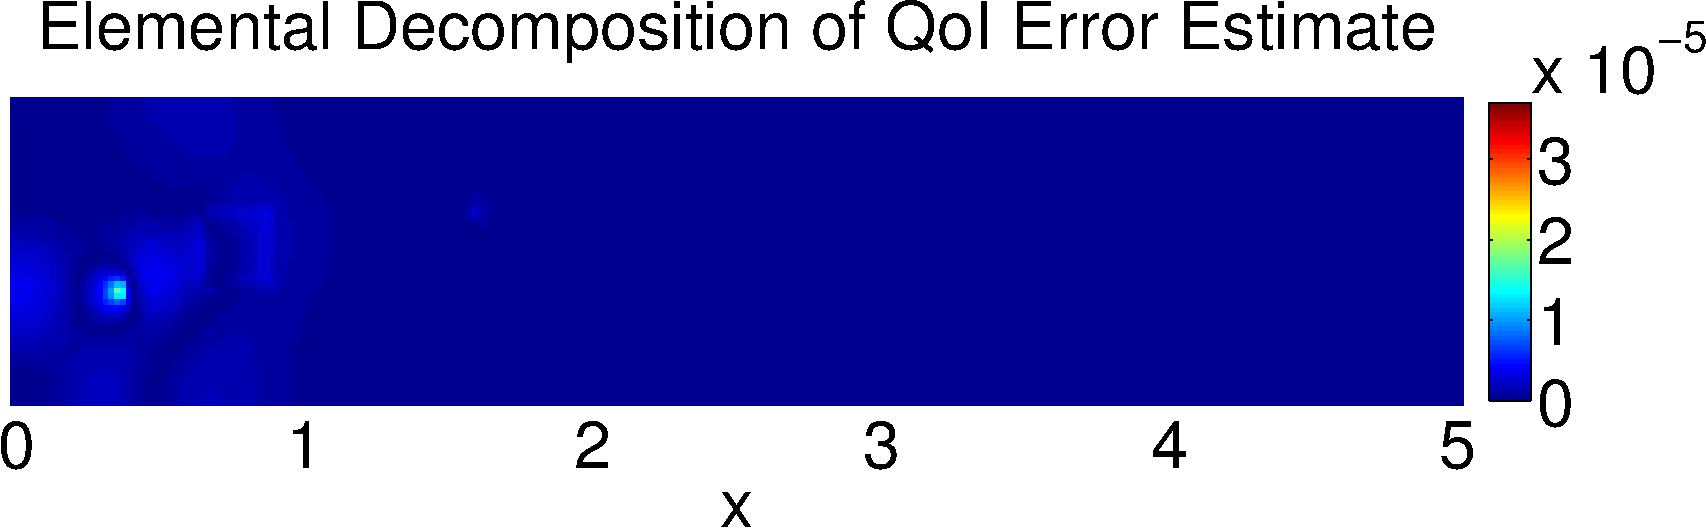
\includegraphics[width=\textwidth]{baseSeries/err_breakdown_MF01.pdf}
    \end{minipage}%
    \hfill
    \begin{minipage}[t]{0.62\textwidth}
      \centering
      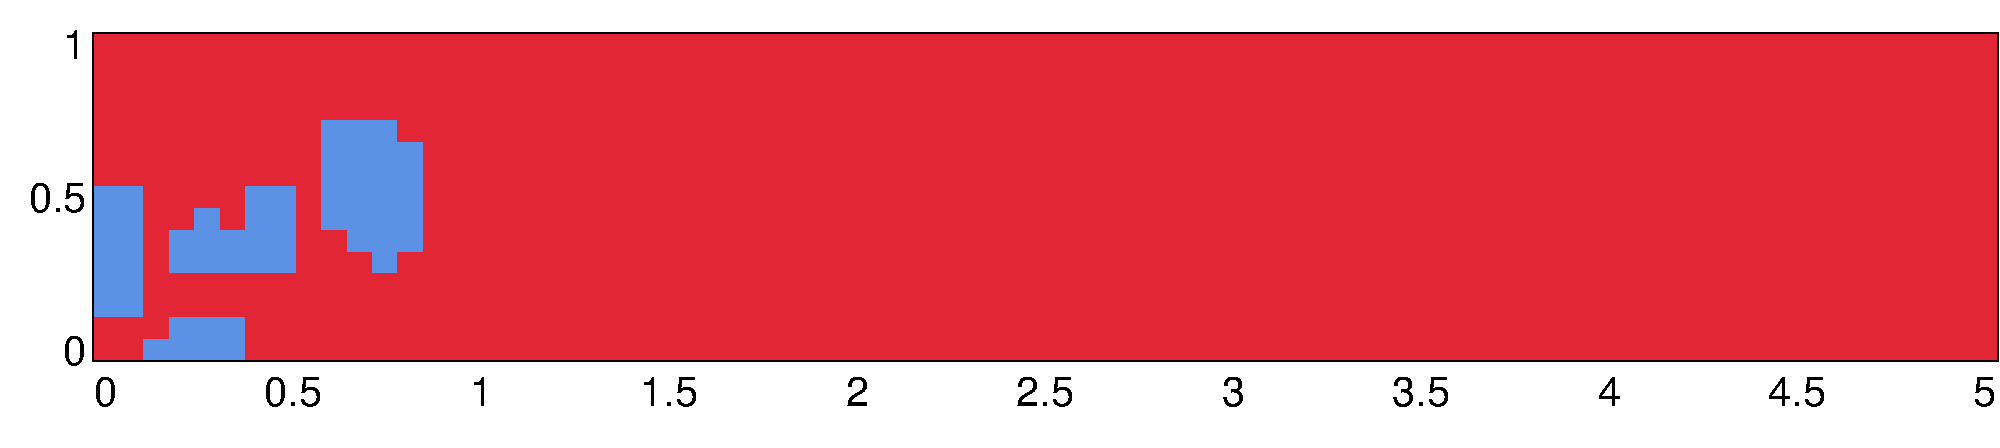
\includegraphics[width=\textwidth]{baseSeries/cd_cdr_MF01_divvy.pdf}
    \end{minipage}%
     }
\makebox[\textwidth]{%
    \begin{minipage}[t]{0.65\textwidth}
      \centering
      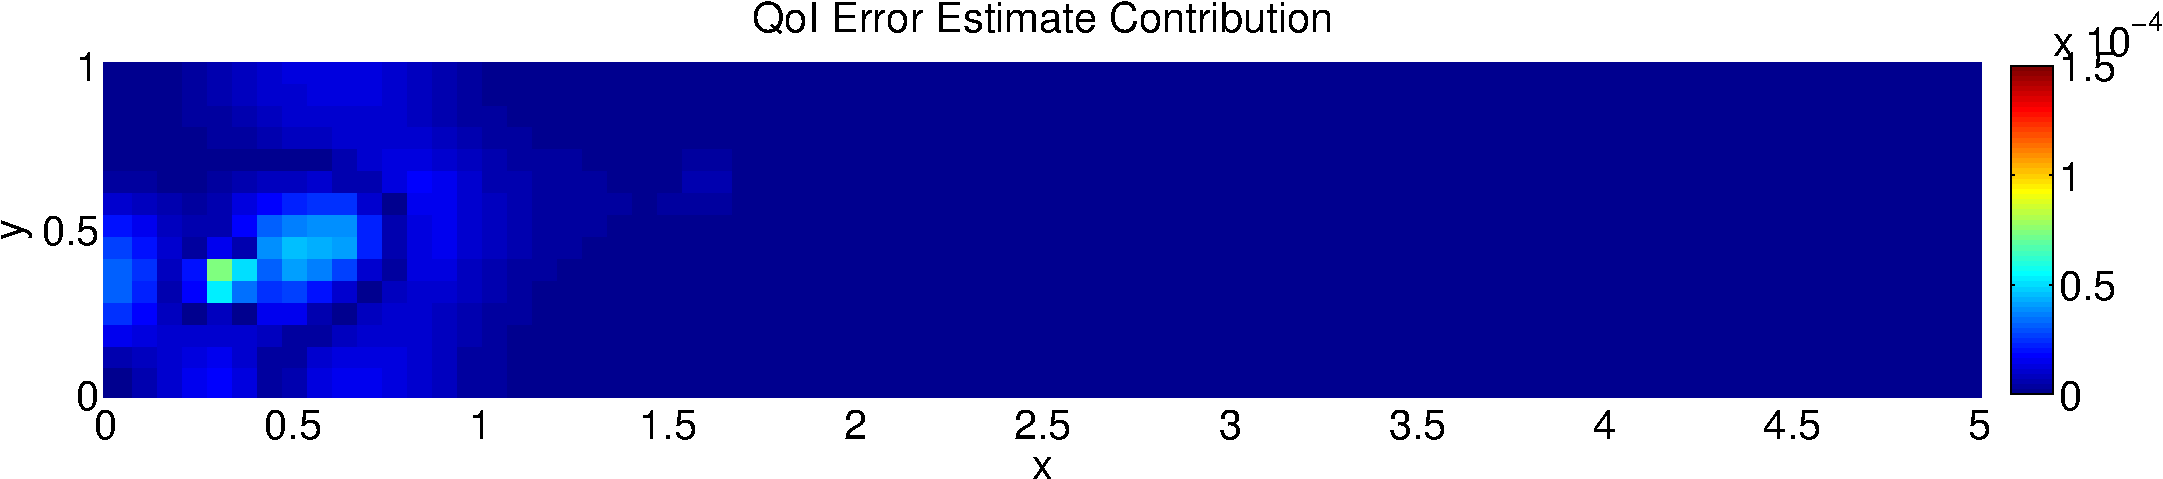
\includegraphics[width=\textwidth]{baseSeries/err_breakdown_MF02.pdf}
    \end{minipage}%
    \hfill
    \begin{minipage}[t]{0.62\textwidth}
      \centering
      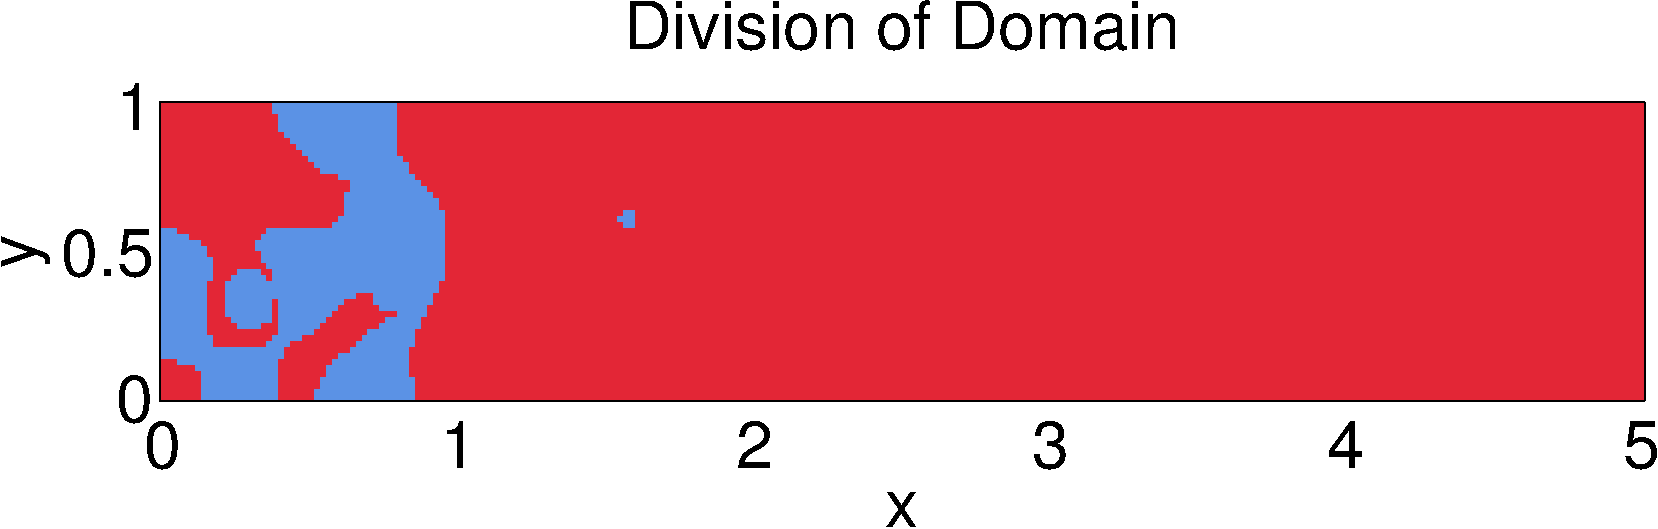
\includegraphics[width=\textwidth]{baseSeries/cd_cdr_MF02_divvy.pdf}
    \end{minipage}%
    }
\makebox[\textwidth]{%
    \begin{minipage}[t]{0.65\textwidth}
      \centering
      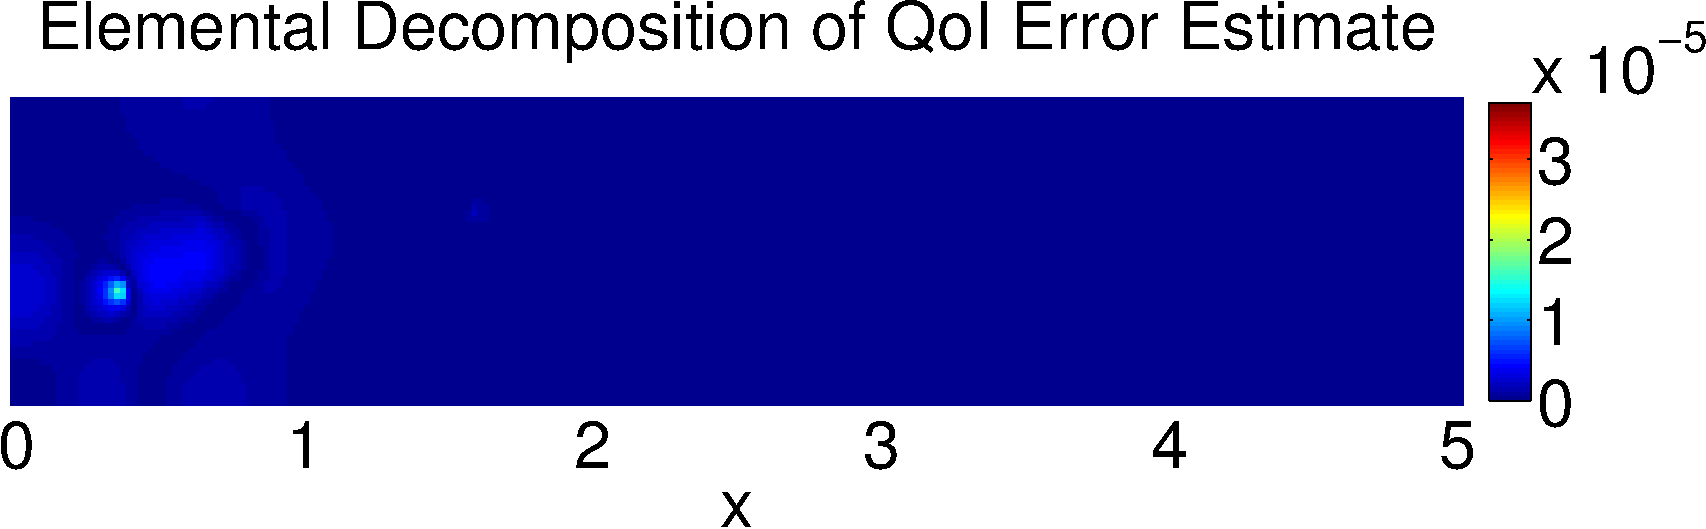
\includegraphics[width=\textwidth]{baseSeries/err_breakdown_MF03.pdf}
    \end{minipage}%
    \hfill
    \begin{minipage}[t]{0.62\textwidth}
      \centering
      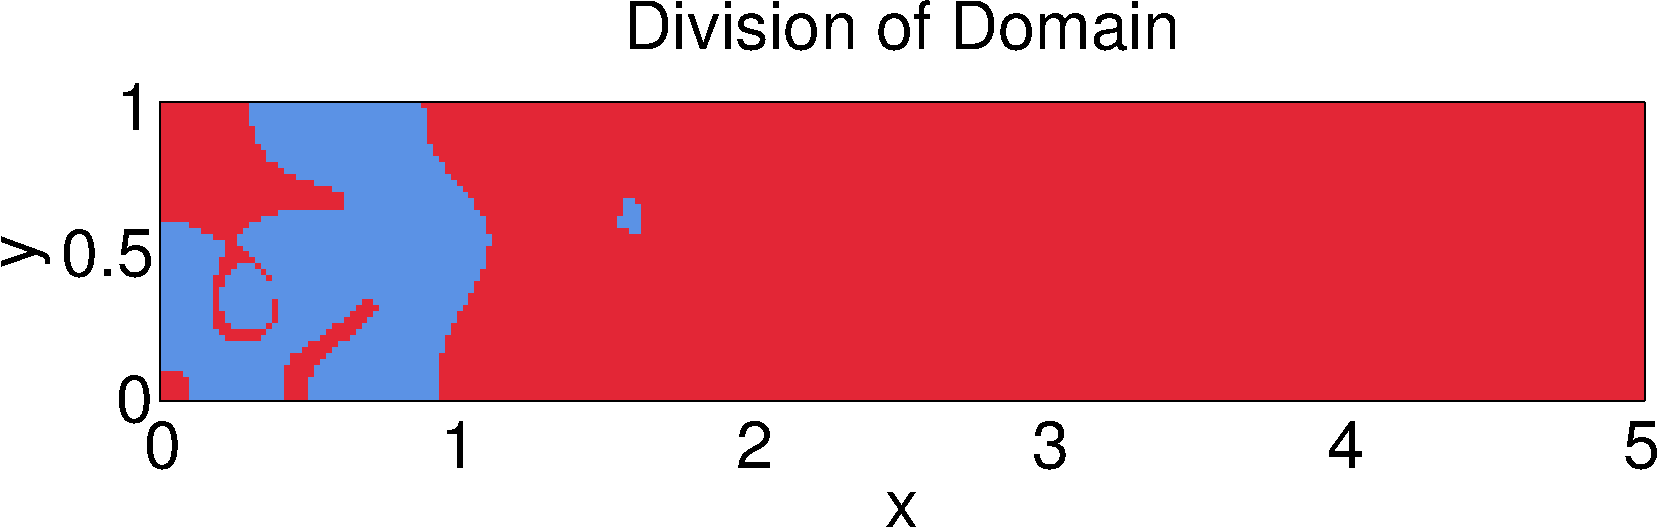
\includegraphics[width=\textwidth]{baseSeries/cd_cdr_MF03_divvy.pdf}
    \end{minipage}%
    }
\makebox[\textwidth]{%
    \begin{minipage}[t]{0.65\textwidth}
      \centering
      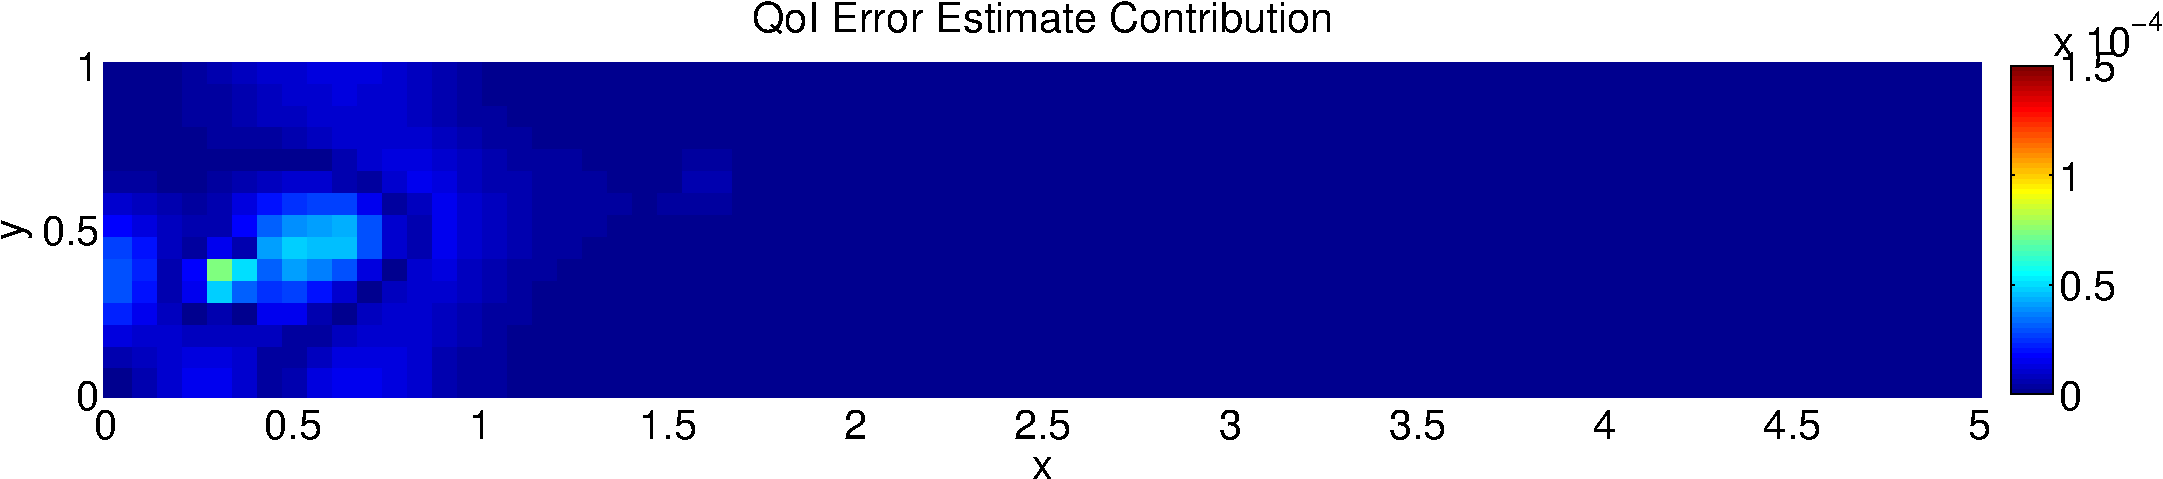
\includegraphics[width=\textwidth]{baseSeries/err_breakdown_MF04.pdf}
    \end{minipage}%
    \hfill
    \begin{minipage}[t]{0.62\textwidth}
      \centering
      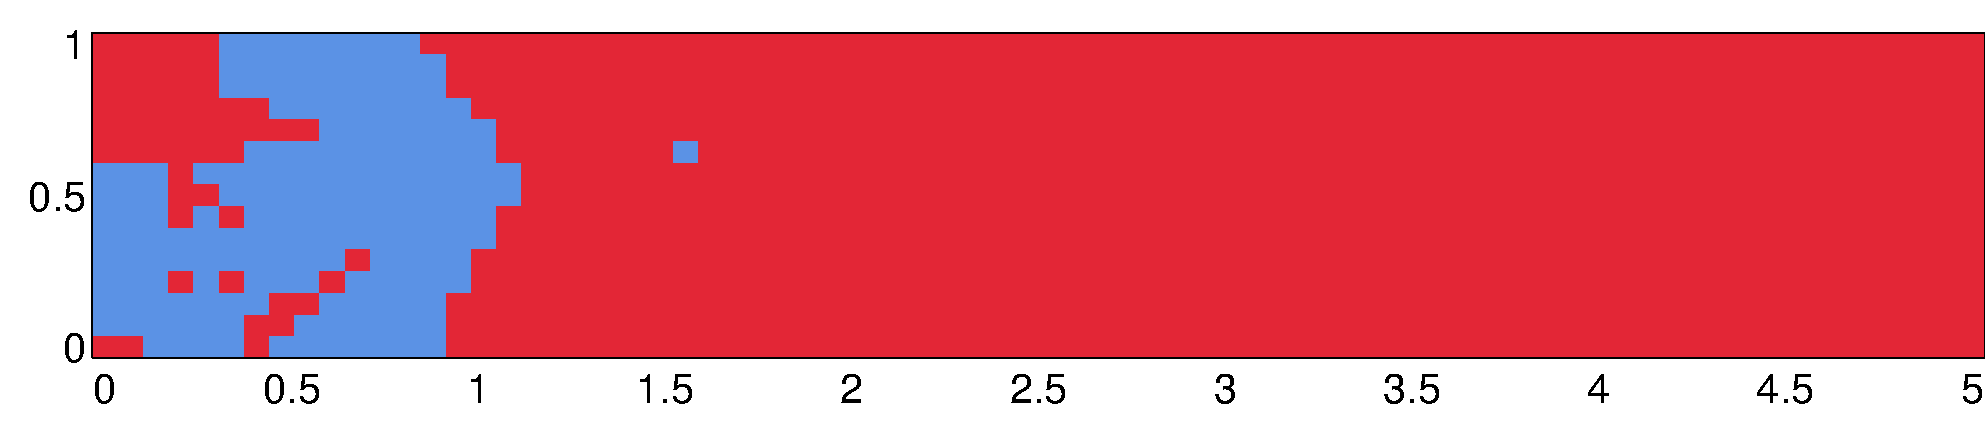
\includegraphics[width=\textwidth]{baseSeries/cd_cdr_MF04_divvy.pdf}
    \end{minipage}%
    }
\makebox[\textwidth]{%
    \begin{minipage}[t]{0.65\textwidth}
      \centering
      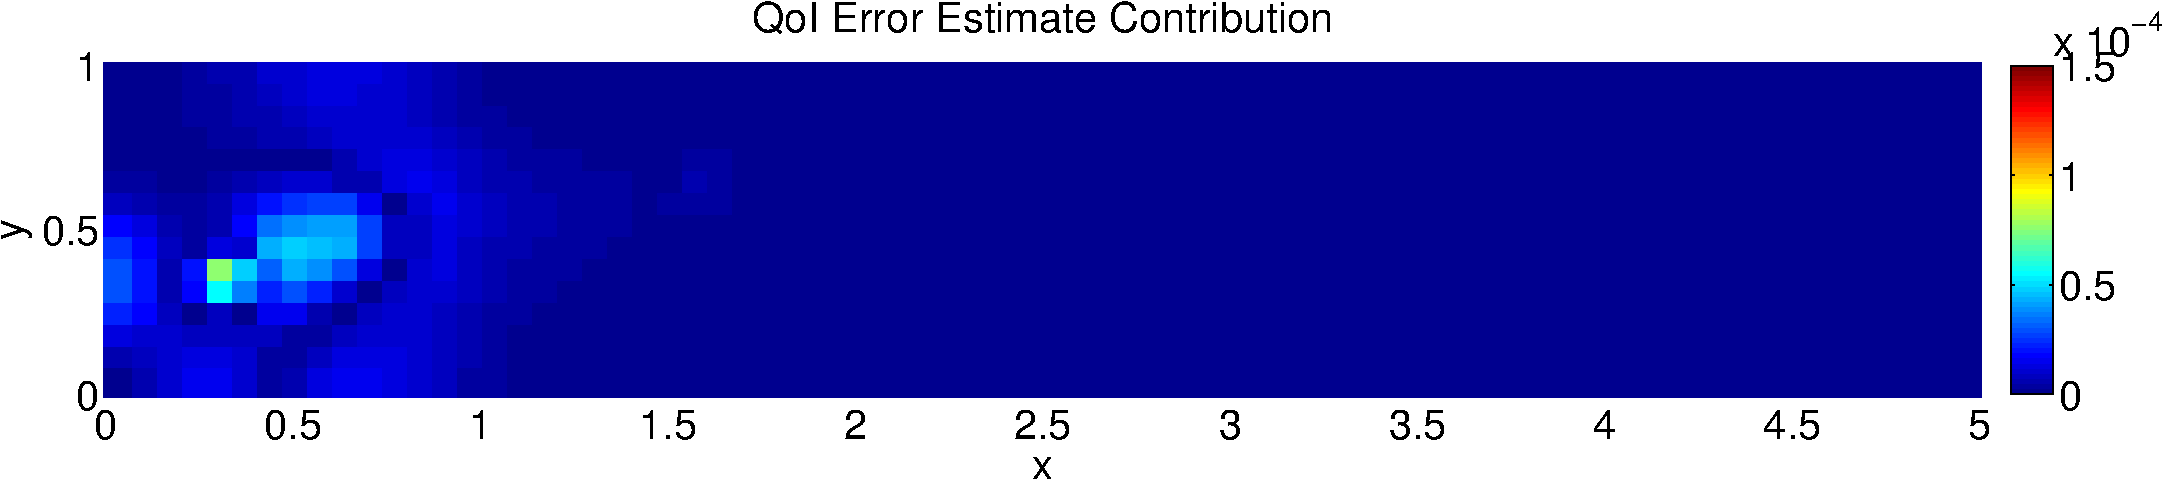
\includegraphics[width=\textwidth]{baseSeries/err_breakdown_MF05.pdf}
    \end{minipage}%
    \hfill
    \begin{minipage}[t]{0.62\textwidth}
      \centering
      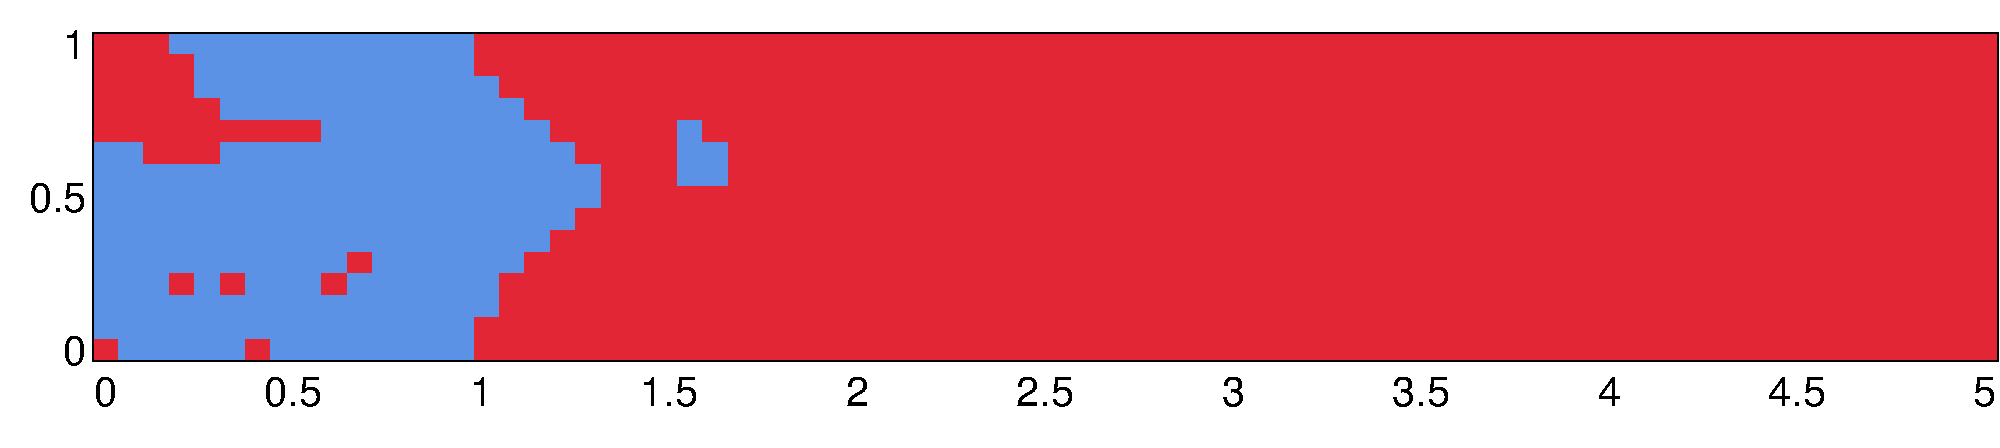
\includegraphics[width=\textwidth]{baseSeries/cd_cdr_MF05_divvy.pdf}
    \end{minipage}%
  }%
\caption{Model refinement series: element-wise breakdown of error estimates and corresponding subdomains (low-fidelity in red, high-fidelity in blue)}
\label{fig:baseRef}
\end{figure}

\begin{figure}[h]
\centering
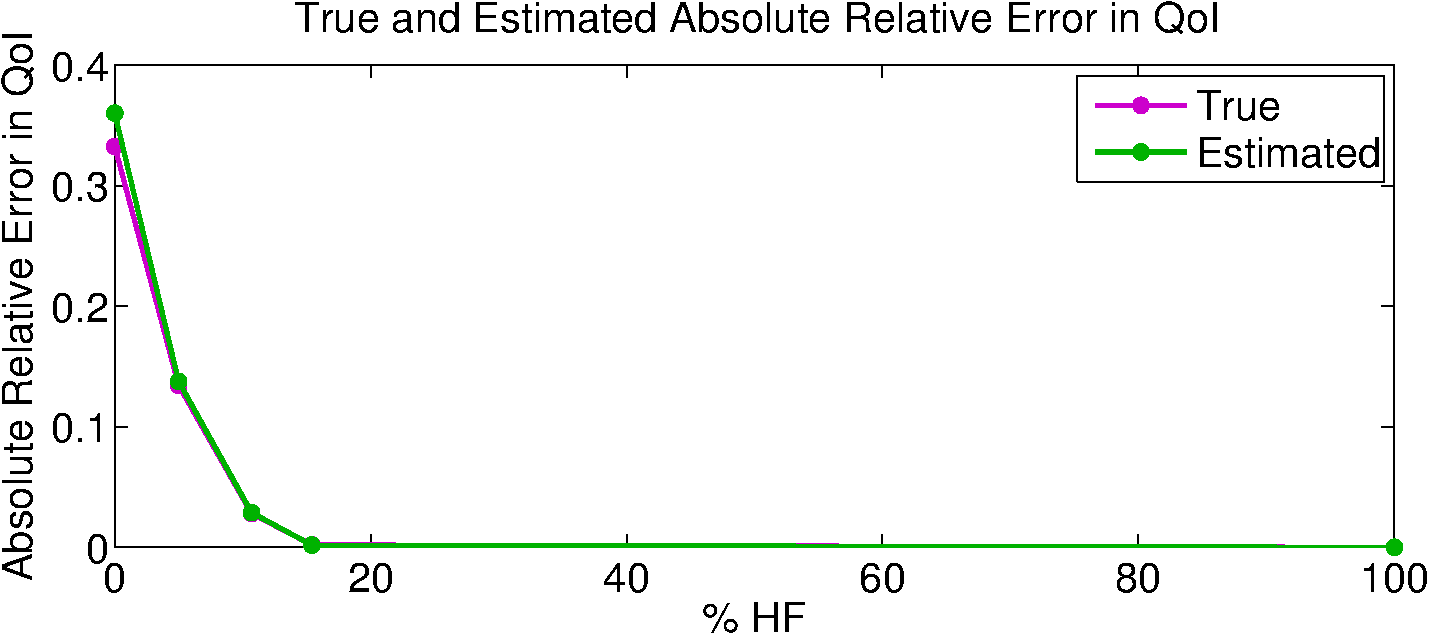
\includegraphics[width=0.8\textwidth]{baseSeries/err_est.pdf}
\caption{True and estimated absolute relative error in QoI}
\label{fig:baseErr}
\end{figure}

\begin{figure}[h]
\centering
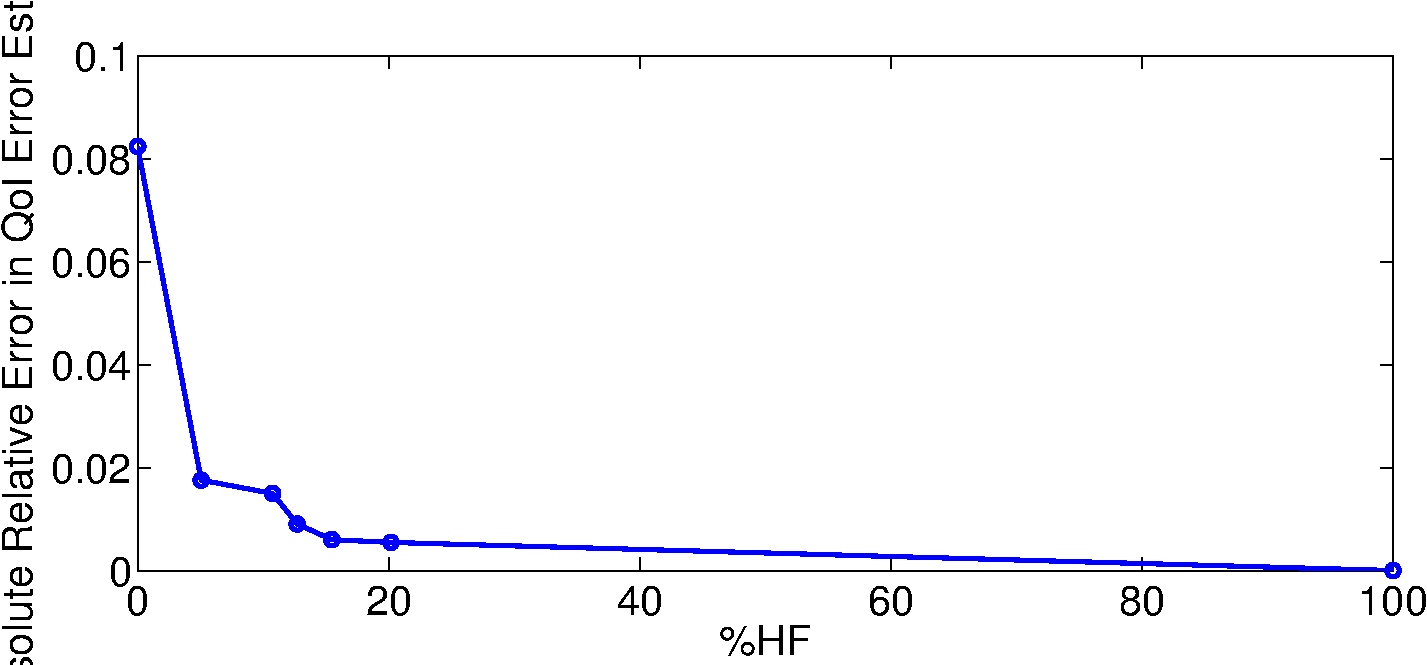
\includegraphics[width=0.8\textwidth]{baseSeries/err_err.pdf}
\caption{Absolute relative error in estimated absolute relative error in QoI \red{replace with table/graph of effectivity indices}}
\label{fig:baseErrErr}
\end{figure}

\subsection{Interaction of Observations and QoI}

The element-wise decomposition of the error estimate (\ref{eq:finErrExp}) suggests the use of the high-fidelity model in areas of the domain where \red{the parameter field?} is both informed by the observations and informative about the QoI. %can we only tie the physical domain and parameters so closely like this because these equations are localized (or what's the word...what hyperbolic equations don't have...something with "local"...)

To see this, we compare the element-wise decomposition of the error estimate for three sizes of the QoI region $\Omega_I$ given the same set of observations, and for three sets of observations given the same QoI region. Only the error estimate linearized about $\Psi_{LF}$ is shown in Figures \ref{fig:qoiStudy} and \ref{fig:dataStudy}; the later estimates have a similarly patterned decomposition.

\begin{figure}
\centering
\subfigure{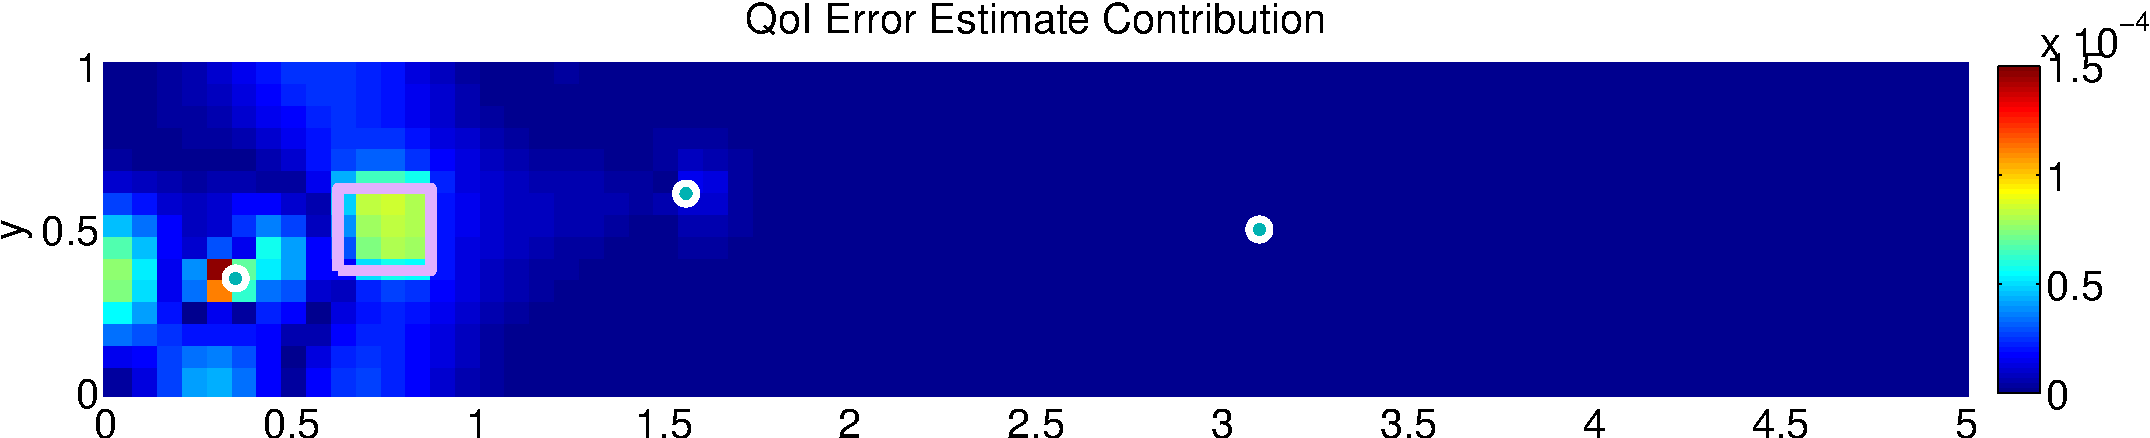
\includegraphics[width=0.8\textwidth]{vs_qoi/err_breakdown_3_3_study.pdf}}
\subfigure{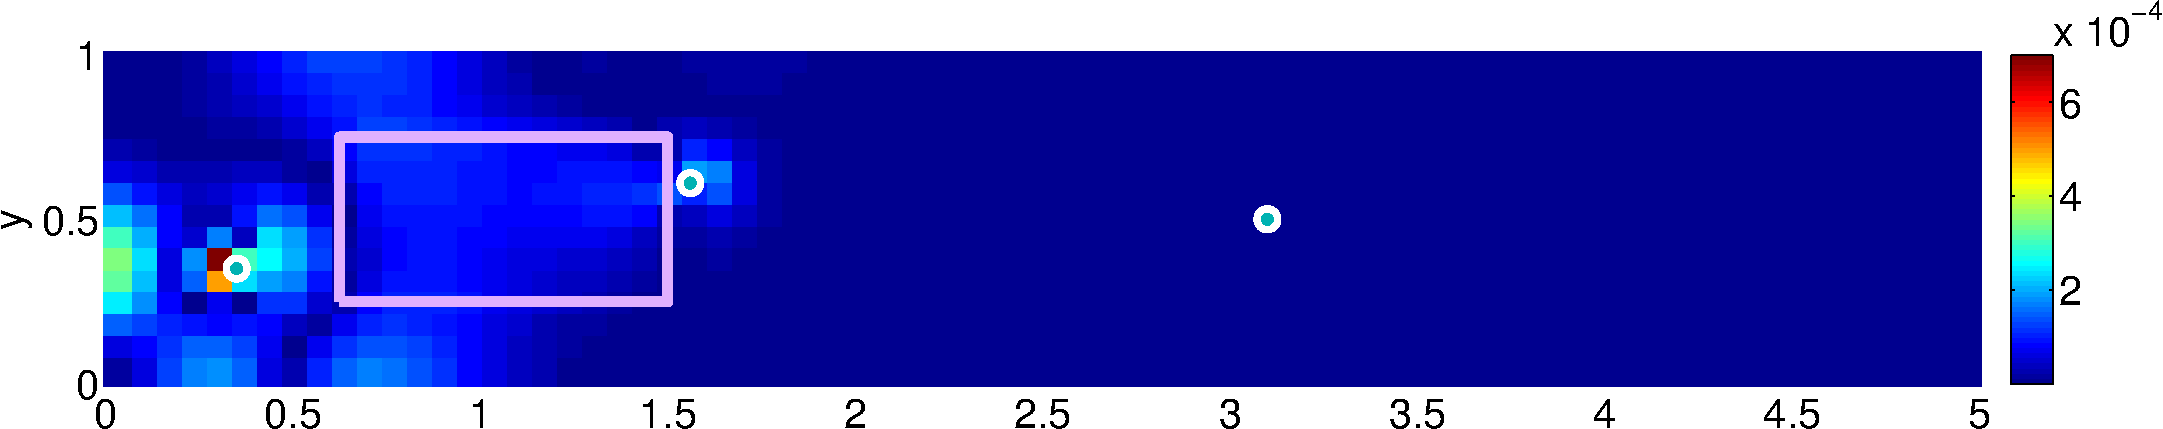
\includegraphics[width=0.8\textwidth]{vs_qoi/err_breakdown_7_3_study.pdf}}
\subfigure{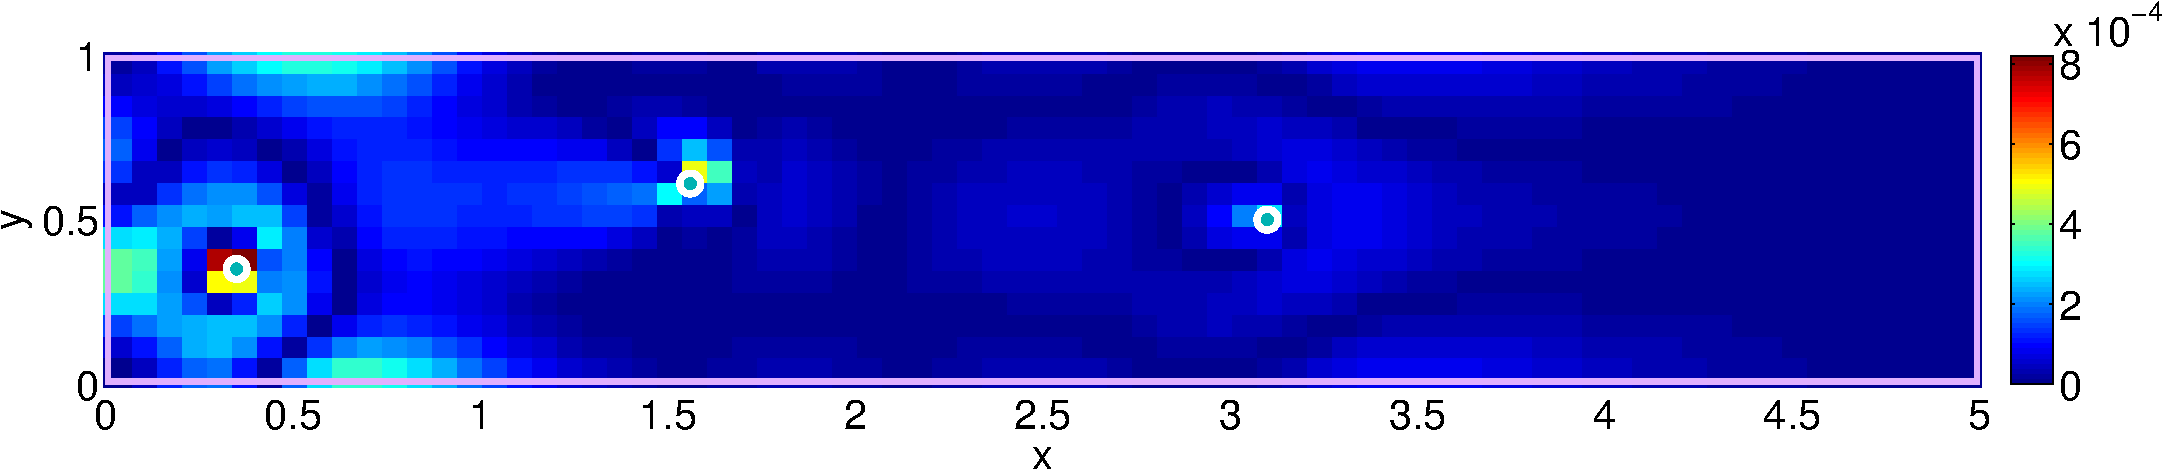
\includegraphics[width=0.8\textwidth]{vs_qoi/err_breakdown_5_3_study.pdf}}
\caption{Element-wise decomposition of error estimates for varying $\Omega_I$ (purple box) and same three observations (teal and white points)}
\label{fig:qoiStudy}
\end{figure}

\begin{figure}
\centering
\subfigure{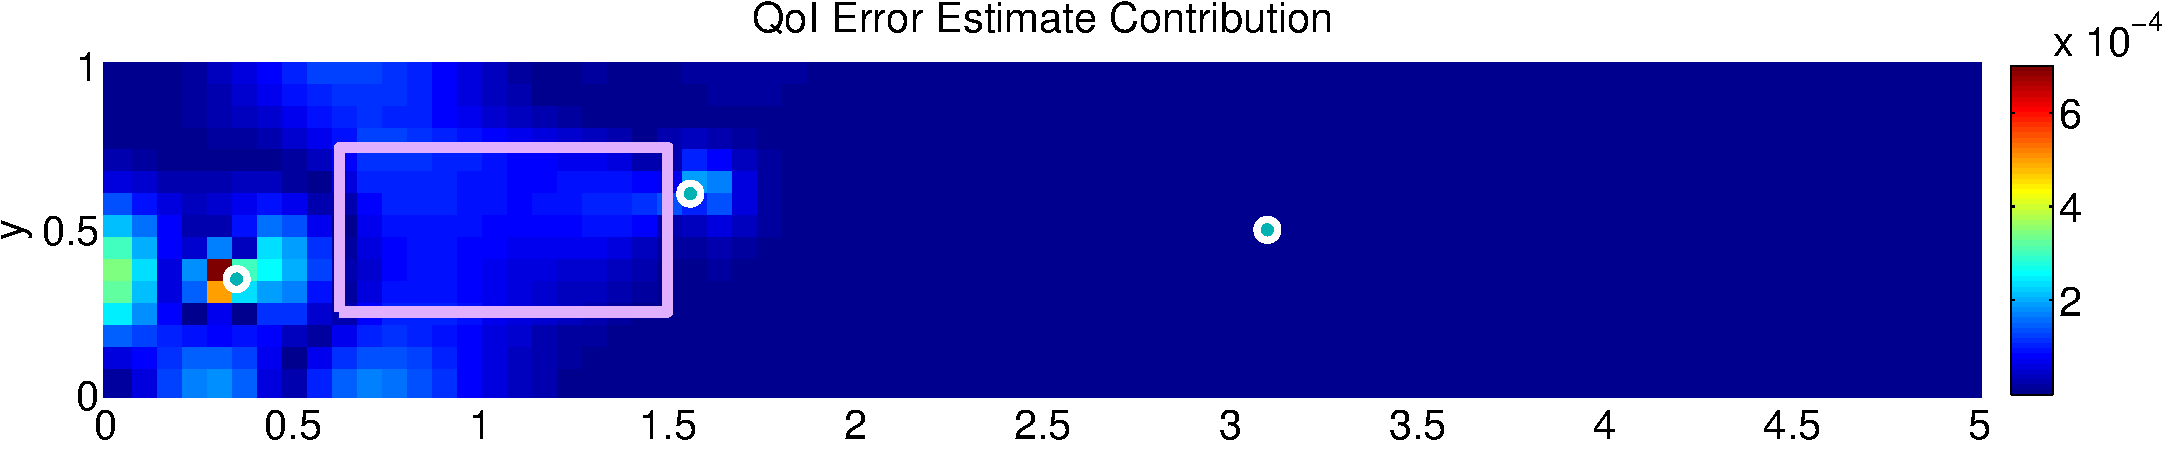
\includegraphics[width=0.8\textwidth]{vs_data/err_breakdown_7_3_studyv2.pdf}}
\subfigure{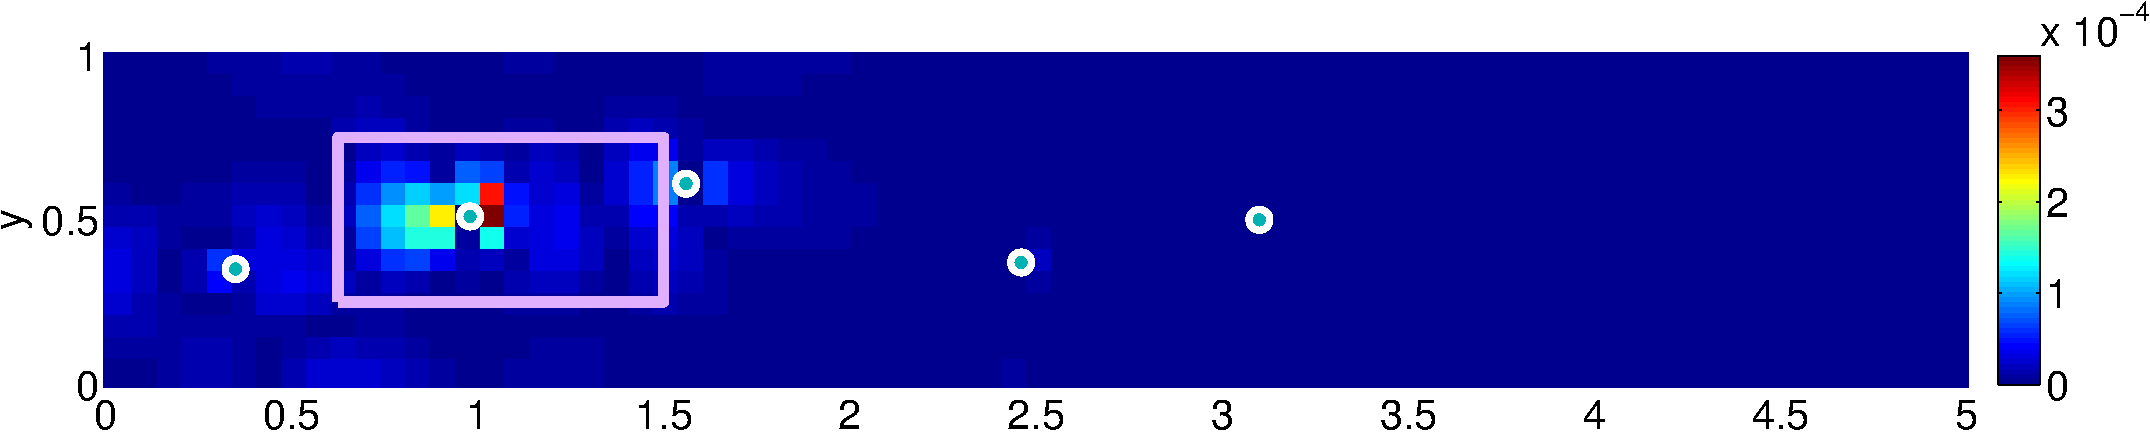
\includegraphics[width=0.8\textwidth]{vs_data/err_breakdown_7_5_study.pdf}}
\subfigure{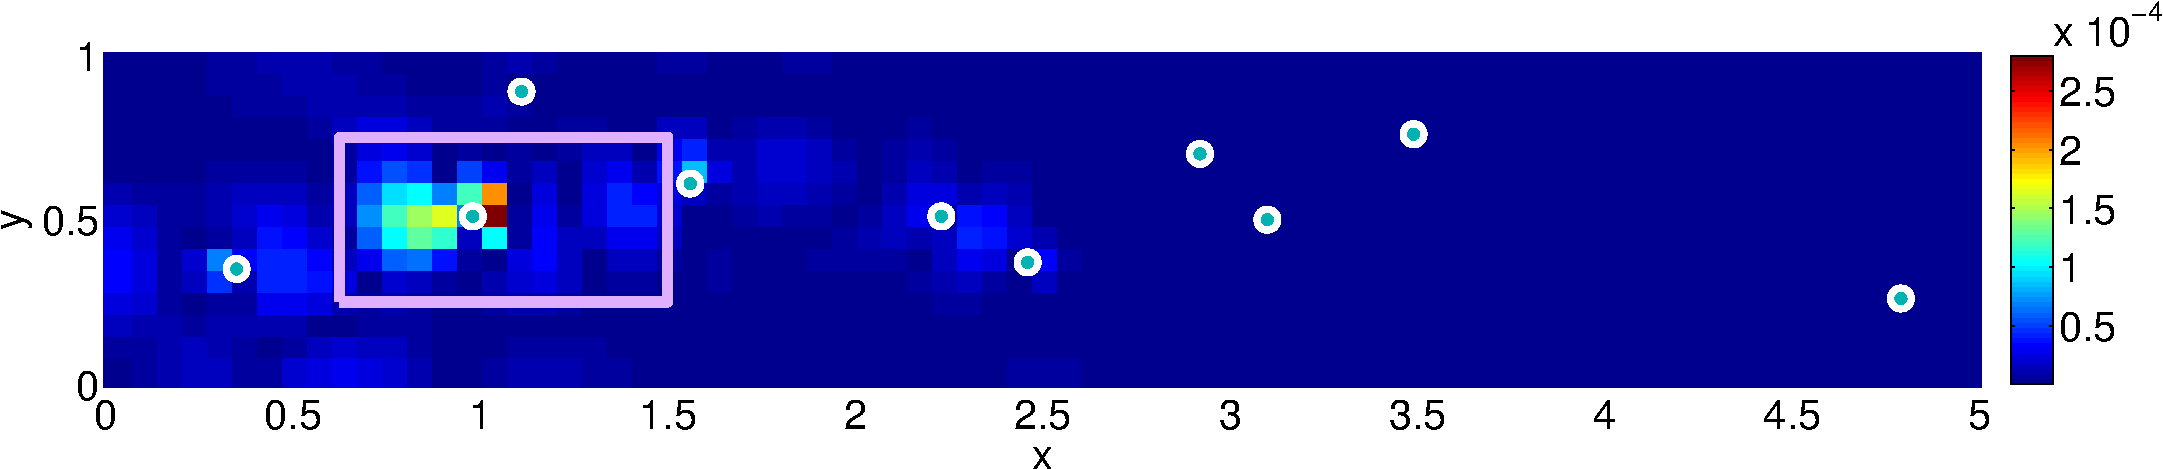
\includegraphics[width=0.8\textwidth]{vs_data/err_breakdown_7_10_study.pdf}}
\caption{Element-wise decomposition of error estimates for varying observations (teal and white points) and same $\Omega_I$ (purple box)}
\label{fig:datStudy}
\end{figure}

These results agree with intuition, and in this case an appropriate mixed-fidelity model could have been designed by intuition. In fact, this is a case in which the models are simple enough that it is actually cheaper to solve the inverse problem with the high-fidelity model than to rigorously form a mixed-fidelity model with which to solve the inverse problem instead. The interaction between the observations and the QoI need not always be obvious, however, as might be the case for \red{what?} models, and it is in these cases that a rigorous method for forming a mixed-fidelity model would be most helpful.

\subsection{Effect of Regularization}

As the magnitude of the regularization parameter $\beta$ it increased, the error estimate seems to indicate that whether the low- or high-fidelity model is used becomes less and less important in most of the domain, except in small areas around the most relevant observations. This behavior is expected\red{, or maybe I've just stared at this too often}. As $\beta$ increases, the regularization more strongly influences the parameter field that is inferred, although the regularization does not completely determine the inferred parameters and the observations still influence the inferred parameter field in the area around them; the choice of model in the QoI region becomes less important as the inferred parameter field in that area becomes more determined by regularization. 

The element-wise decomposition for the observations and QoI region shown in Figure \ref{fig:baseSetup} are shown in Figure \ref{fig:regStudy} for three values of the regularization parameter $\beta$. Only the error estimate linearized about $\Psi_{LF}$ is shown; the later estimates have a similarly patterned decomposition.

\begin{figure}
\centering
\subfigure{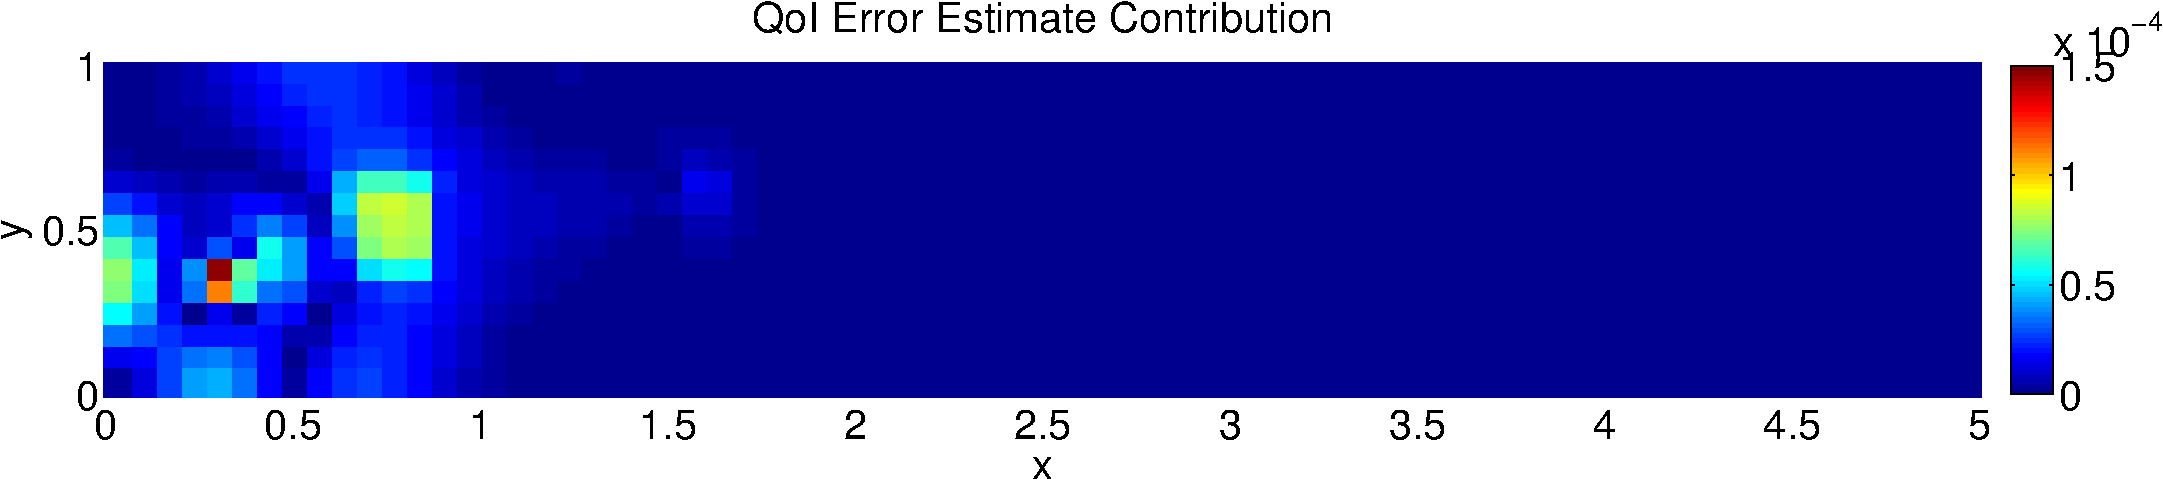
\includegraphics[width=0.8\textwidth]{vs_reg/err_breakdown_0p00001.pdf}}
\subfigure{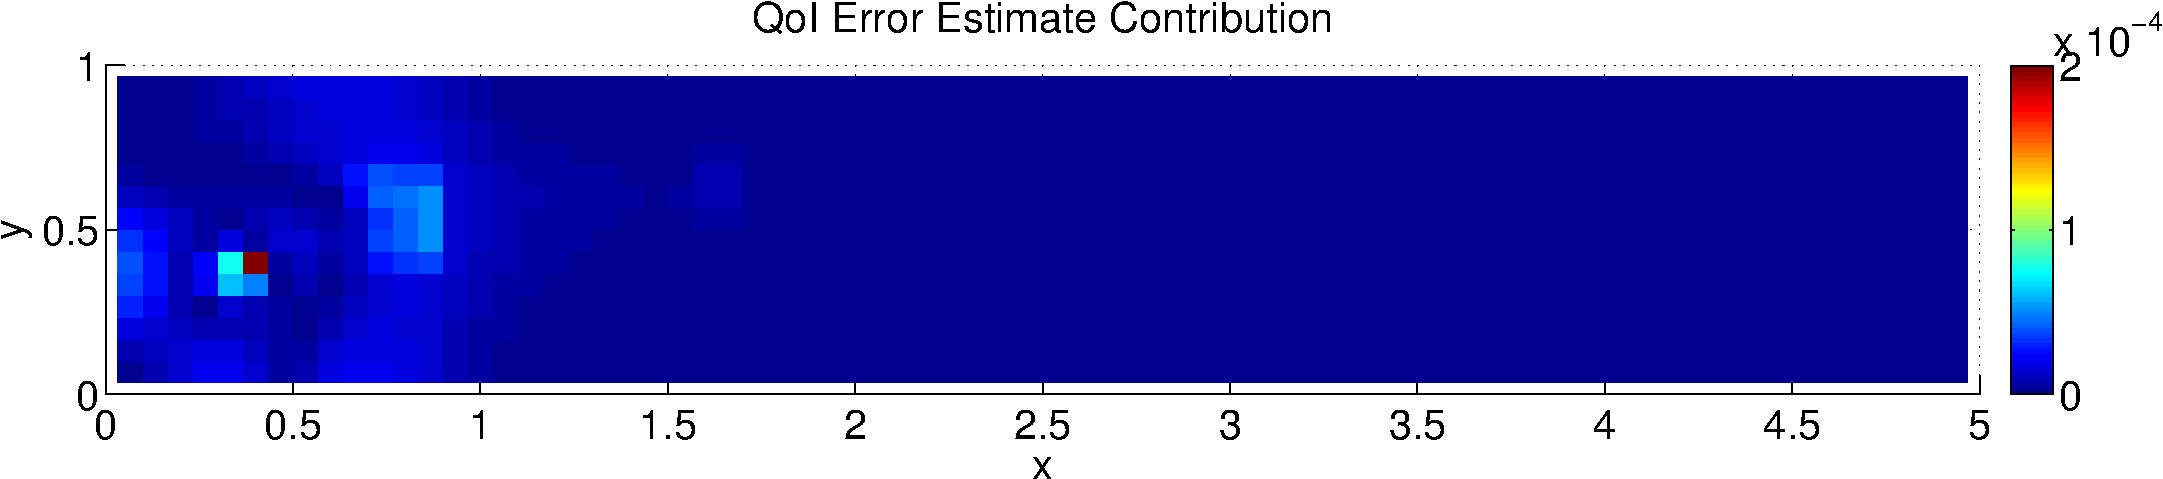
\includegraphics[width=0.8\textwidth]{vs_reg/err_breakdown_0p001.pdf}}
\subfigure{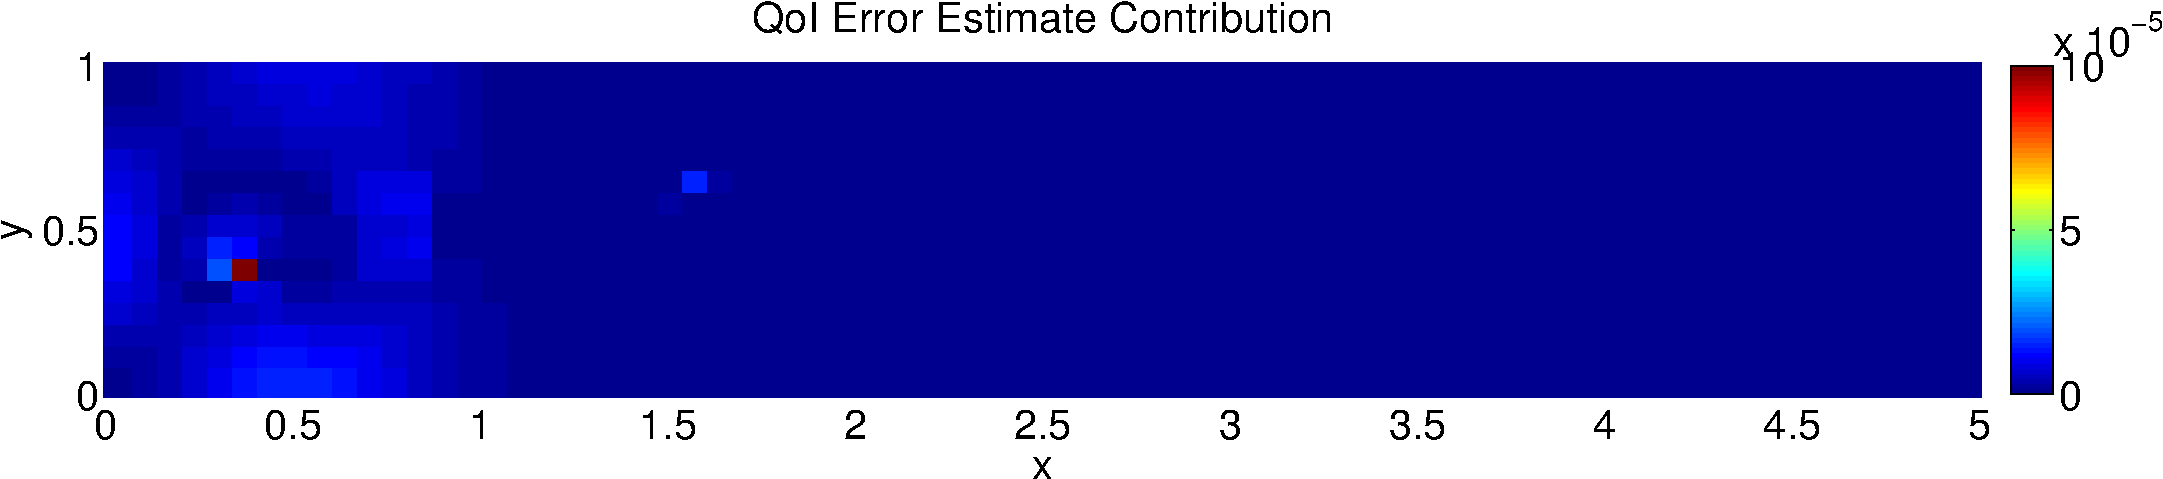
\includegraphics[width=0.8\textwidth]{vs_reg/err_breakdown_0p1.pdf}}
\caption{Element-wise decomposition of error estimates for varying $\beta$ \red{if keep make consistent}}
\label{fig:regStudy}
\end{figure}

%how to show, since a paper can't include animations or their flip-book equivalent? if showing how it picks out the important data points, how to justify only showing one (and not all from series of refinements), since linearization could contaminate error breakdown...
% -> vs measurements studies; vs qoi studies; vs reg study (?)
% -> DON'T HAVE: looking at contribution from regularization terms? indicator function QoI? boundary flux QoI? more physically meaningful boundary conditions? *different physics, one where effects propogate more*? 
	
%effectivity index (ratio of estimated to true error) plots/tables? (oden, prudhomme, et al mention such)

%...relate back to Chad's subspace of shared qoi-data importance (emphasis on shared importance...)? although his subspace was in parameter-space, not physical domain space...
%can we make an example where the qoi region is not pointed out for refinement? even with weak regularization

%try runs with inflow boundary conditions, which make more sense?
%gunzburger only has example with homo diri around the entire boundary...how to deal with BCs if boundary split between diri and neumann? -> poke 930...

%should these be re-run on finer meshes for prettier pictures?

%------------------------------------------------------------------------------%
\section{Scalar versus Field Parameters}  %\label{sec:xx}
%------------------------------------------------------------------------------%

The models considered need not differ in the physics included. In this section, we consider two models which differ in the space in the space to which the parameter belongs. The high-fidelity model 
\begin{equation}
k_d\nabla^2 u - \vec{V}\cdot\nabla u + k_ru^2= f(q),\quad q\in U,
\end{equation}
is again a single-species convection-diffusion-reaction equation with a nonlinear reaction term, where $k_d = 0.1$ is a diffusion coefficient and $k_r = -4.2$ is a reaction coefficient. The low-fidelity model
\begin{equation}
k_d\nabla^2 u - \vec{V}\cdot\nabla u + k_ru^2= f(q),\quad q\in\R
\end{equation}
differs from the high-fidelity model only in that the parameter is a scalar instead of a field.

%effect of linearization? the third point popping in and out in 4p2_deref is probably due to interplay of how fast third point's bump shrinks versus how fast the refinement percentage grows...
%can philisohically compare with chad's though, perhaps in param refinement, even though his is in parameter subspaces and ours is in physical space?

\chapter{Conclusion}
%------------------------------------------------------------------------------%
\section{Future Work}  \label{sec:xx}
%------------------------------------------------------------------------------%

%stochastic
%wolfgang and bangert -> mesh refinement and stochastic, keep coarse sometimes...see if this might be related to extension?


%theory and numerical results section...start writing up theory, nevermind flow? and outline of which numerical results? include discussion of costs? error bounds? section for limitations (what models, linearization, anything else in possible quals questions chew)? pictures of auxiliary variables? extension to more than two models?
% -> vs measurements studies; vs qoi studies; vs reg study (?); effect of linearization?
% -> DON'T HAVE: looking at contribution from regularization terms? indicator function QoI? *different physics, one where effects propogate more*? *transient*?
%formulation for altobjfx was just what chad said; you just implemented it for a toy problem to see what would happen

\appendix
\chapter{Notation} \label{appendix}

For quick reference, the following table summarizes notation used throughout this thesis 
(in alphabetical order).

\begin{table}[!ht]
\caption{Summary of Notation}
\begin{center}
\begin{tabular}{c|l}
\textbf{Symbol} & \textbf{Meaning} \\
\hline \hline
$q$  &   Model parameters \\
$u$  &   Model state\\
\end{tabular}
\end{center}
\end{table}

%% This defines the bibliography file (main.bib) and the bibliography style.
%% If you want to create a bibliography file by hand, change the contents of
%% this file to a `thebibliography' environment.  For more information 
%% see section 4.3 of the LaTeX manual.
\begin{singlespace}
\addcontentsline{toc}{chapter}{\hspace{3ex}Bibliography}
\bibliography{masterBib}
\bibliographystyle{plain}
\end{singlespace}

\end{document}
